\documentclass[a4paper,openright,12pt]{book}
\usepackage[spanish]{babel} % espanol
\usepackage{fancyhdr}
\usepackage{lastpage}
\usepackage{graphicx} % graficos
\usepackage{hyperref}
\usepackage[utf8]{inputenc}
\usepackage{enumerate}


% nivel que se numera y aparece en el indice
\setcounter{secnumdepth}{3}
\setcounter{tocdepth}{3}

% quitar el 0.
\renewcommand\thesection{\arabic{section}}

% tabla de contenidos como seccion
\makeatletter
\renewcommand\tableofcontents{
    \section*{{Tabla de contenidos} %linea importante
        \@mkboth{
           \MakeUppercase\contentsname}{\MakeUppercase\contentsname}}
    \@starttoc{toc}
    }
\makeatother

% bibliografia como seccion
\makeatletter
\renewenvironment{thebibliography}[1]{
     \section*{Bibliografía} %linea importante
      \@mkboth{\MakeUppercase\bibname}{\MakeUppercase\bibname}
      \list{\@biblabel{\@arabic\c@enumiv}}
           {\settowidth\labelwidth{\@biblabel{#1}}
            \leftmargin\labelwidth
            \advance\leftmargin\labelsep
            \@openbib@code
            \usecounter{enumiv}
            \let\p@enumiv\@empty
            \renewcommand\theenumiv{\@arabic\c@enumiv}}
      \sloppy
      \clubpenalty4000
      \@clubpenalty \clubpenalty
      \widowpenalty4000
      \sfcode`\.\@m}
     {\def\@noitemerr
       {\@latex@warning{Empty `thebibliography' environment}}
      \endlist}
\makeatother

% aqui definimos el encabezado
\lhead[\thepage/\pageref{LastPage}]{}
\chead[Informe]{Informe}
\rhead[]{\thepage/\pageref{LastPage}}
\renewcommand{\headrulewidth}{0.5pt}

% aqui definimos el pie de pagina
\lfoot[EPIS]{Base de Datos II}
\cfoot[\today]{\today}
\rfoot[Base de Datos II]{EPIS}
\renewcommand{\footrulewidth}{0.5pt}

\pagestyle{fancy} 

% margenes
\setlength{\oddsidemargin}{5mm}
\setlength{\evensidemargin}{5mm}

\begin{document}

\begin{titlepage}
\begin{center}
\begin{figure}[htb]
\begin{center}

\includegraphics[width=4cm]{./images/upt}
\end{center}
\end{figure}

UNIVERSIDAD PRIVADA DE TACNA\\
\vspace*{0.10in}
FACULTAD DE INGENIERIA\\
Escuela Profesional de Ingeniería de Sistemas\\
\vspace*{0.2in}
\begin{large}
TEMA : \\
\end{large}
\vspace*{0.2in}
\begin{Large}
\textbf{PRACTICAS DE LABORATORIO} \\
\end{Large}
\vspace*{0.3in}
\begin{large}
DOCENTE: PATRICK CUADROS QUIROGA\\
\end{large}
\vspace*{0.3in}
\rule{80mm}{0.1mm}\\
\vspace*{0.1in}
\begin{large}
PRESENTADO POR: \\
Jose Luis Condori Choquecota \\
Elisban Vilca Mamani\\
Gary Calle Cortez (2013000664)

\end{large}
\rule{80mm}{0.1mm}\\
\begin{large}
2017\\
\end{large}
\end{center}
\end{titlepage}


\tableofcontents
\pagenumbering{arabic}
\lhead[\thepage/\pageref{LastPage}]{\thesection. Tabla de contenidos}
\rhead[\thesection. Tabla de contenidos]{\thepage/\pageref{LastPage}}
\newpage



\section{4-1 Ejercicio 0: Instalacion de Oracle SQL Devevloper Data Modeler}\label{se:nudo}
\lhead[\thepage/\pageref{LastPage}]{\thesection. Nudo}
\rhead[\thesection. Nudo]{\thepage/\pageref{LastPage}}
Descripción general\\
En esta práctica,se instalaran Oracle SQL Develouper Data Modeler. Siga las instrucciones en funcion de si dispone de un sistema operativo Windows, Mac o Linux.\\
Tareas:
\begin{enumerate}
    \item Ingresamos a la página web de Oracle.
    \item Descargamos el programa, aceptamos la licencia y Descargamos el programa .
    \item Ejecutamos el programa..
\end{enumerate}
\begin{center}
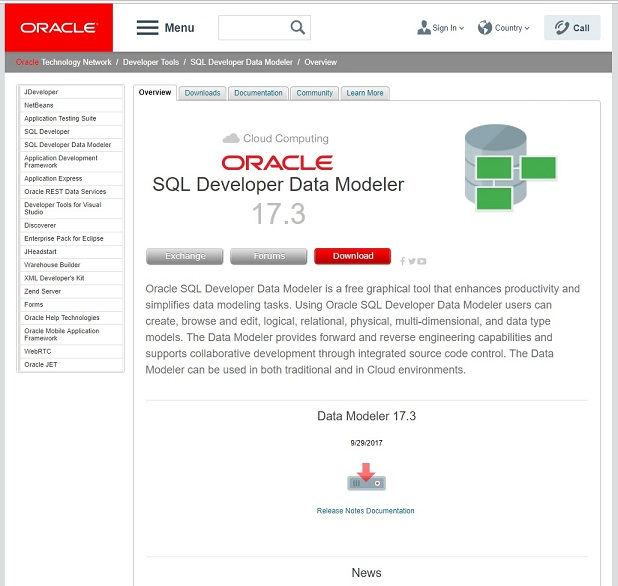
\includegraphics[scale=1]{Imag04/1.jpg}\\
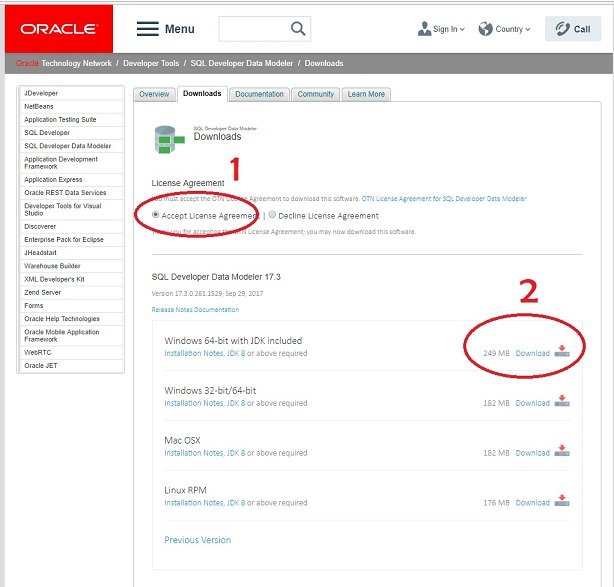
\includegraphics[scale=1]{Imag04/2.jpg}\\
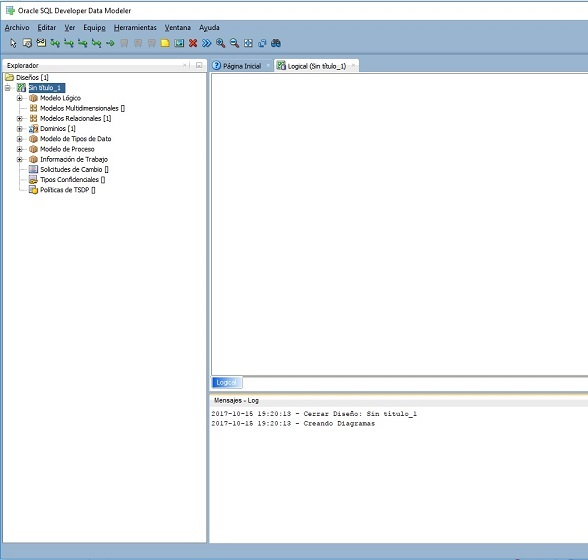
\includegraphics[scale=1]{Imag04/3.jpg}\\
\end{center}

\section{4-1 Ejercicio 1: Identificacion y Creacion de Entidades y Atributos}\label{se:nudo}
\lhead[\thepage/\pageref{LastPage}]{\thesection. Nudo}
\rhead[\thesection. Nudo]{\thepage/\pageref{LastPage}}
Descripción general\\
En esta práctica, identificará y modelará las entidades y los atributos de una base de datos académica o, en otras palabras, un sistema de gestión de escuela.\\
Tareas:\\
Para su comodidad, aquí se muestra un resumen de cómo funciona la base de datos académica (sistema de gestión de escuela):\\

a. Una escuela/universidad tiene diferentes departamentos que ofrecen cursos a los alumnos en una determinada sesión académica. 

b. Cada uno de estos cursos lo imparte un profesor. 

c. Los alumnos pueden inscribirse en diferentes cursos en una sesión académica. 

d. Además de los detalles de registro, la universidad/escuela debe mantener también la información principal sobre el alumno. 

e. El departamento mantiene los detalles de asistencia del alumno, que determinarán si un alumno puede optar a los exámenes de esa sesión académica o no.
 
f. Para cada sesión académica, se realizan exámenes y los resultados se comparten con el alumno en un período de tiempo estipulado.
 
g. El departamento también mantiene un registro del tiempo de conexión y desconexión del profesorado para sus necesidades de generación de informes.\\ 

Con la información proporcionada anteriormente, utilice Oracle SQL Developer Data Modeler para identificar y crear:\\ 

Las entidades del sistema de gestión de escuela 

Los atributos para cada una de las entidades indicadas
 
La relación entre las entidades\\
\begin{center}
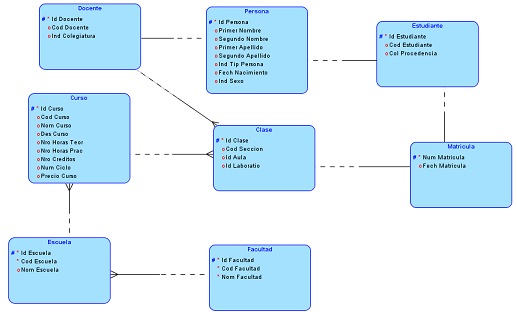
\includegraphics[scale=1]{Imag04/4.png} 
\end{center}

\section{4-2 Ejercicio 1: Ingenieria Directa de un Modelo Logico en un Modelo Relacional}\label{se:nudo}
\lhead[\thepage/\pageref{LastPage}]{\thesection. Nudo}
\rhead[\thesection. Nudo]{\thepage/\pageref{LastPage}}
Descripción general\\
En esta práctica realizará ingeniería directa del modelo lógico de la base de datos académica en un modelo relacional con Oracle SQL Developer Data Modeler.\\
Tareas:\\

1. Para realizar la ingeniería directa del modelo lógico de la base de datos académica a un modelo relacional, realice lo siguiente: \\

a. Abra el modelo lógico en Oracle SQL Developer Data Modeler 

b. Haga clic en el icono Engineer to Relational Model. 

c. Acepte todos los valores por defecto y haga clic en Engineer. 

d. Expanda el nodo Relational Models en el explorador de objetos para ver los objetos creados\\
\begin{center}
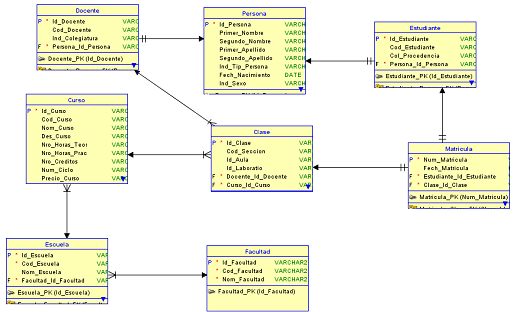
\includegraphics[scale=1]{Imag04/5.png} 
\end{center}

\section{4-2 Ejercicio 2: Ingenieria Inversa de un Modelo Relacional en un Modelo Logico}\label{se:nudo}
\lhead[\thepage/\pageref{LastPage}]{\thesection. Nudo}
\rhead[\thesection. Nudo]{\thepage/\pageref{LastPage}}
Descripción general\\
En esta práctica, agregará una nueva columna al modelo relacional de ingeniería en la práctica y, a continuación, realizará ingeniería inversa del modelo relacional en el modelo lógico.\\
Tareas:\\

Agregue una columna a una de las tablas del modelo relacional. En la siguiente captura de pantalla, la columna  se agrega a la tabla . 

Ahora, para realizar la ingeniería inversa del modelo relacional de la base de datos académica a un modelo lógico con los cambios, realice lo siguiente:\\ 

a. Haga clic en el icono Engineer to Logical Model. 

b. Acepte todos los valores por defecto y haga clic en Engineer.
 
c. Verifique si el nuevo atributo se ha agregado al modelo lógico.\\
\begin{center}
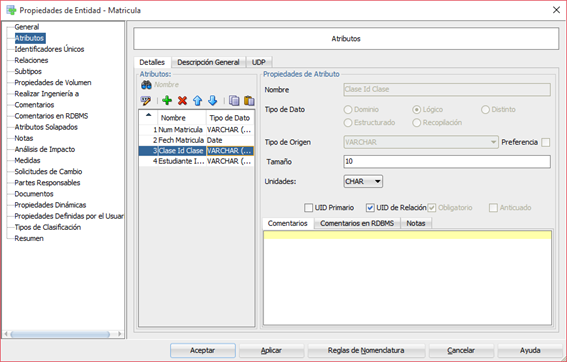
\includegraphics[scale=1]{Imag04/6.png} 
\end{center}


\section{5-1 Ejercicio 1: Creación de un Glosario a Partir del Modelo Lógico}\label{se:nudo}
\lhead[\thepage/\pageref{LastPage}]{\thesection. Nudo}
\rhead[\thesection. Nudo]{\thepage/\pageref{LastPage}}
Descripción general\\
En esta práctica, creará un glosario a partir del modelo lógico de la base de datos académica.\\
Tareas
\begin{enumerate}
    \item Abra el modelo lógico de la base de datos académica.
    \item Haga clic con el botón derecho en el nodo Logical Model en el explorador y seleccione "Create Glossary from Logical Model".
    \item Especifique el nombre del glosario, una breve descripción y tantos tipos de clasificación como sean aplicables a las entradas del glosario.
    \item Guarde el glosario.
\end{enumerate}
\begin{center}
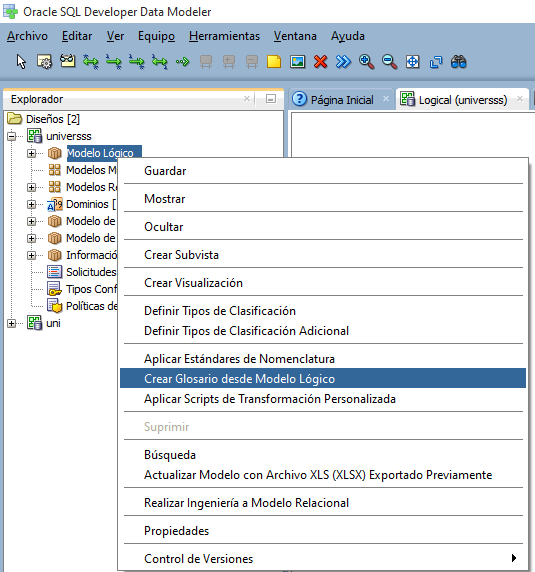
\includegraphics[width=11cm]{./images/5-1 Ejercicio 1/1.png}\\
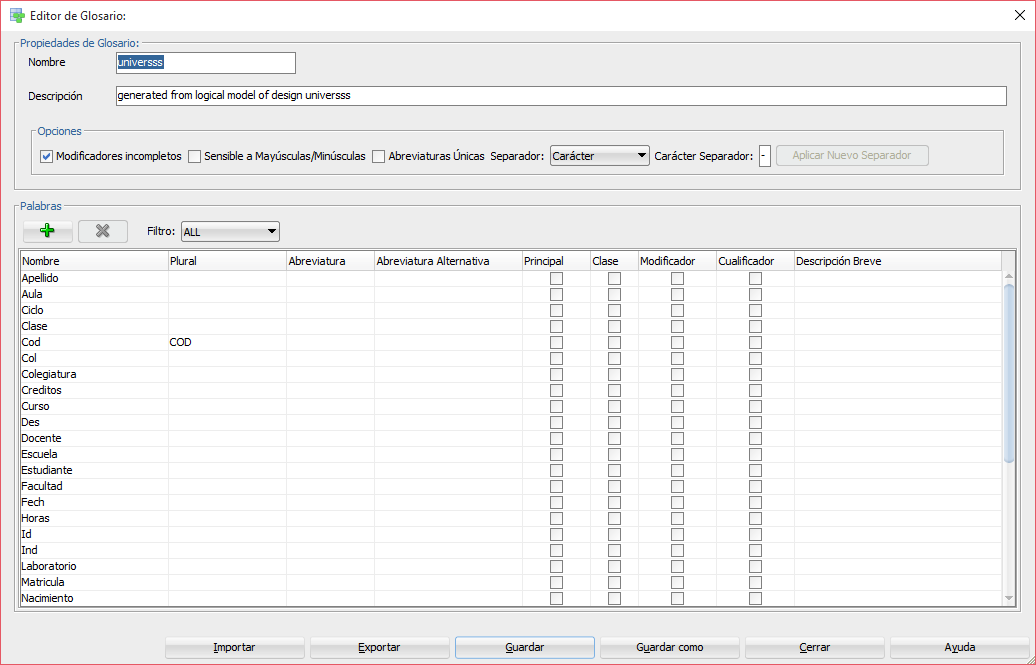
\includegraphics[width=17cm]{./images/5-1 Ejercicio 1/2.png}\\
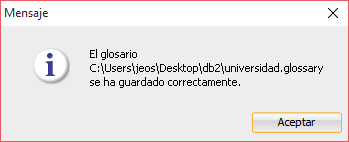
\includegraphics[width=12cm]{./images/5-1 Ejercicio 1/3.png}\\
\end{center}



\section{5-1 Ejercicio 2: Creación de un Archivo.csv con Nombres Predefinidos}\label{se:nudo}
\lhead[\thepage/\pageref{LastPage}]{\thesection. Nudo}
\rhead[\thesection. Nudo]{\thepage/\pageref{LastPage}}
Descripción general\\
En esta práctica, creará un archivo .csv con abreviaturas de los nombres predefinidos que se utilizarán en el modelo relacional de la base de datos académica.\\
Tareas
\begin{enumerate}
\item  Haga clic en Tools > Name Abbreviations.
\item Especifique el archivo .csv que contiene los pares de valores separados por comas.
\item Especifique los objetos a los que se aplicarían los cambios de nombre.
\item Especifique si se mantendrán las mayúsculas o minúsculas del nombre actual al cambiar la cadena de nombre
\end{enumerate}
\begin{center}
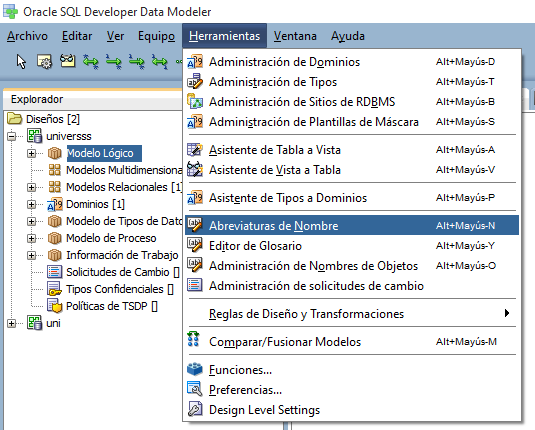
\includegraphics[width=11cm]{./images/5-1 Ejercicio 2/1.png}\\
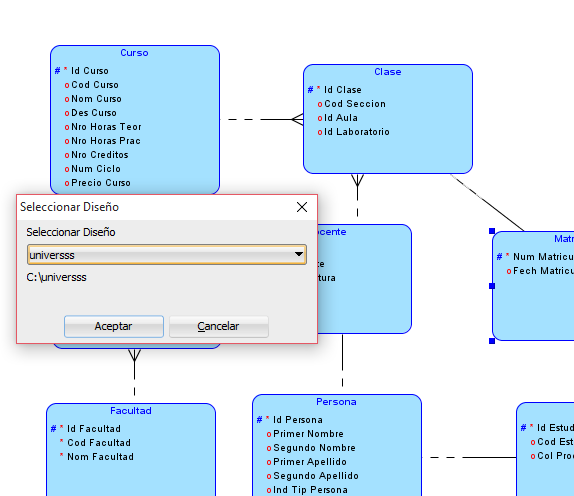
\includegraphics[width=11cm]{./images/5-1 Ejercicio 2/2.png}\\
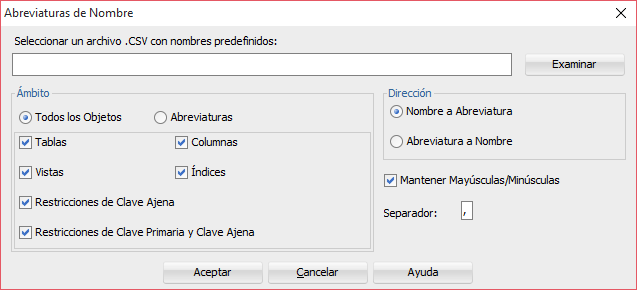
\includegraphics[width=14cm]{./images/5-1 Ejercicio 2/3.png}\\
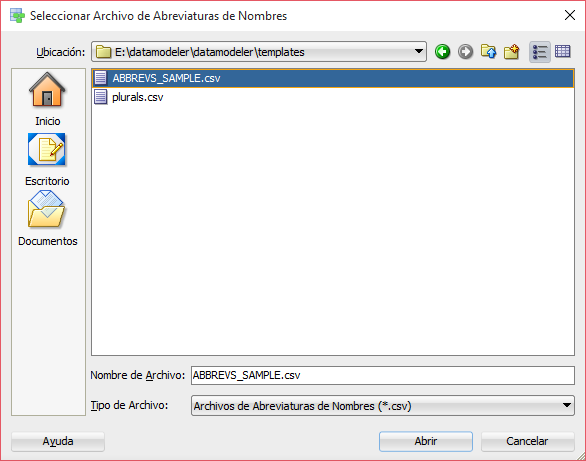
\includegraphics[width=11cm]{./images/5-1 Ejercicio 2/4.png}\\
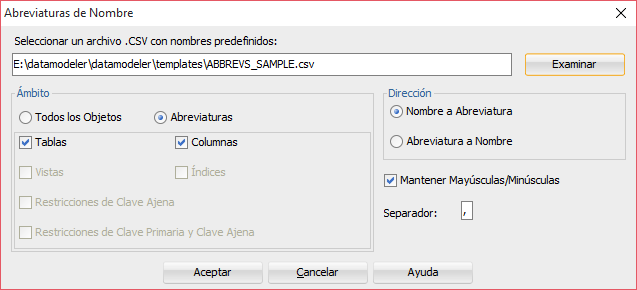
\includegraphics[width=11cm]{./images/5-1 Ejercicio 2/5.png}\\
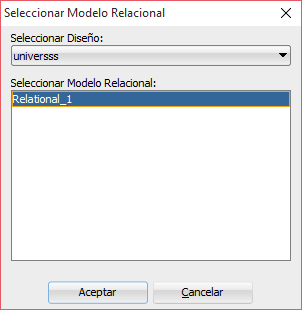
\includegraphics[width=10cm]{./images/5-1 Ejercicio 2/6.png}\\
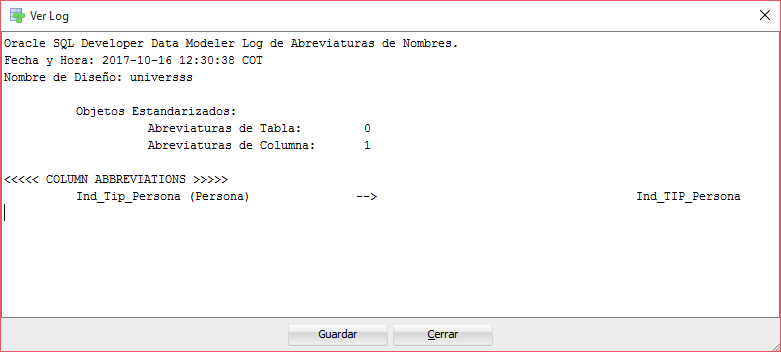
\includegraphics[width=14cm]{./images/5-1 Ejercicio 2/7.png}\\
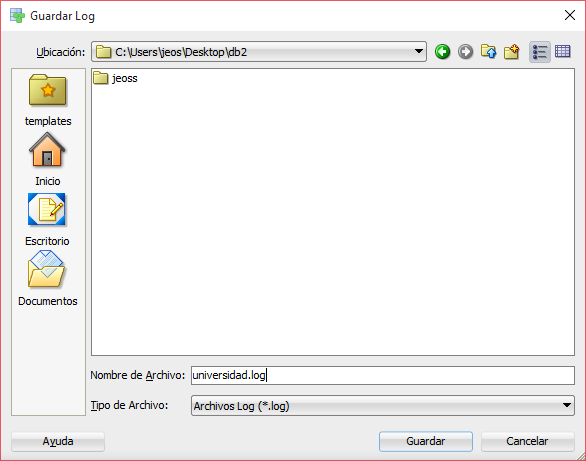
\includegraphics[width=11cm]{./images/5-1 Ejercicio 2/8.png}\\
\end{center}



\section{5-1 Ejercicio 3: Creación de un Juego de Reglas}\label{se:nudo}
\lhead[\thepage/\pageref{LastPage}]{\thesection. Nudo}
\rhead[\thesection. Nudo]{\thepage/\pageref{LastPage}}
Descripción general\\
En esta práctica, creará un juego de reglas para la base de datos académica.\\
Tareas\\
Para crear un juego de reglas, realice los siguientes pasos:\\
\begin{enumerate}
\item Seleccione Design Rules en el menú Tools.
\item Haga clic en el separador Rule Set y, a continuación, en el icono Add Rule Set (signo más).
\item Especifique un nombre para el grupo de reglas.
\item Haga clic en el icono de lápiz Rule Set Properties.
\item Utilice el cuadro de diálogo Rule Set Properties para mover las reglas deseadas de la columna All Rules a la columna Selected Rules.
\item Una vez realizada esta operación, seleccione "Apply Selected RuleSet" para aplicar el juego de reglas seleccionado al diseño actual
\end{enumerate}
\begin{center}
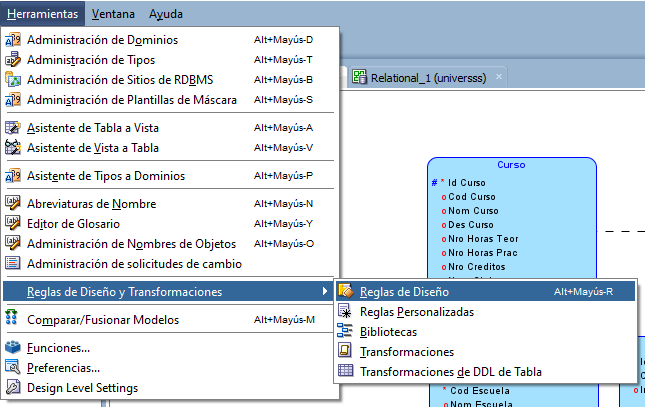
\includegraphics[width=11cm]{./images/5-1 Ejercicio 3/1.png}\\
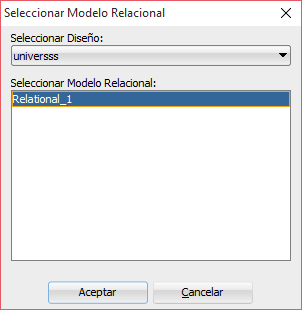
\includegraphics[width=11cm]{./images/5-1 Ejercicio 3/2.png}\\
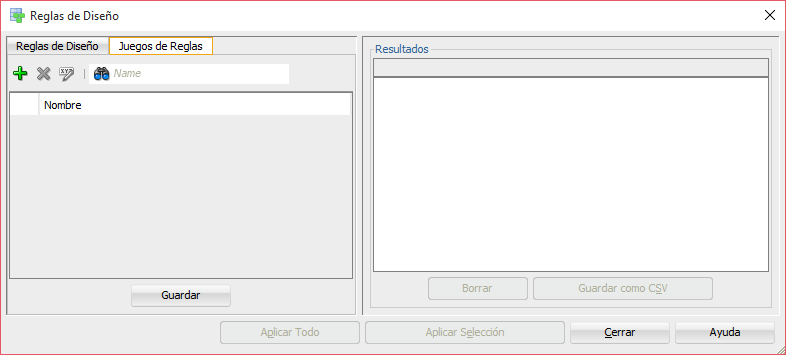
\includegraphics[width=11cm]{./images/5-1 Ejercicio 3/3.png}\\
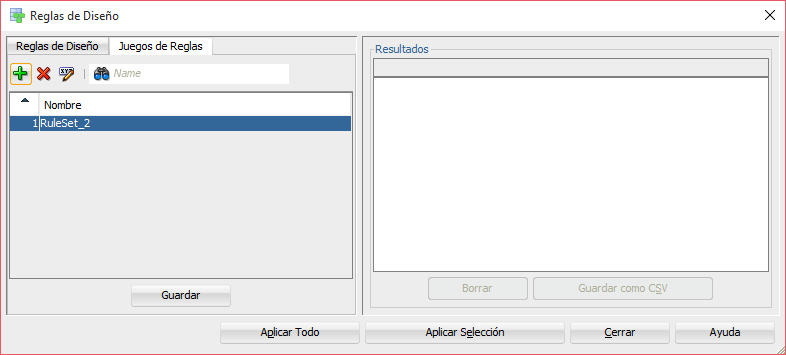
\includegraphics[width=11cm]{./images/5-1 Ejercicio 3/4.png}\\
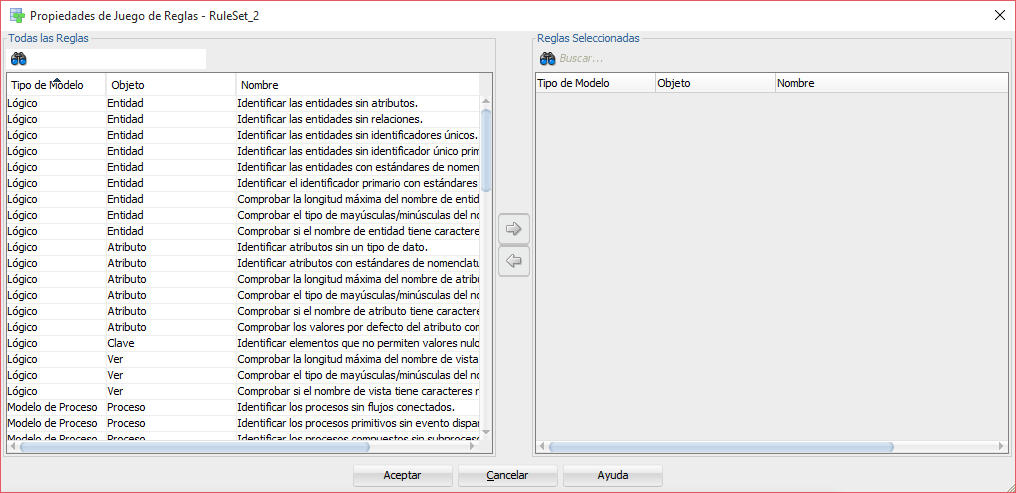
\includegraphics[width=11cm]{./images/5-1 Ejercicio 3/5.png}\\
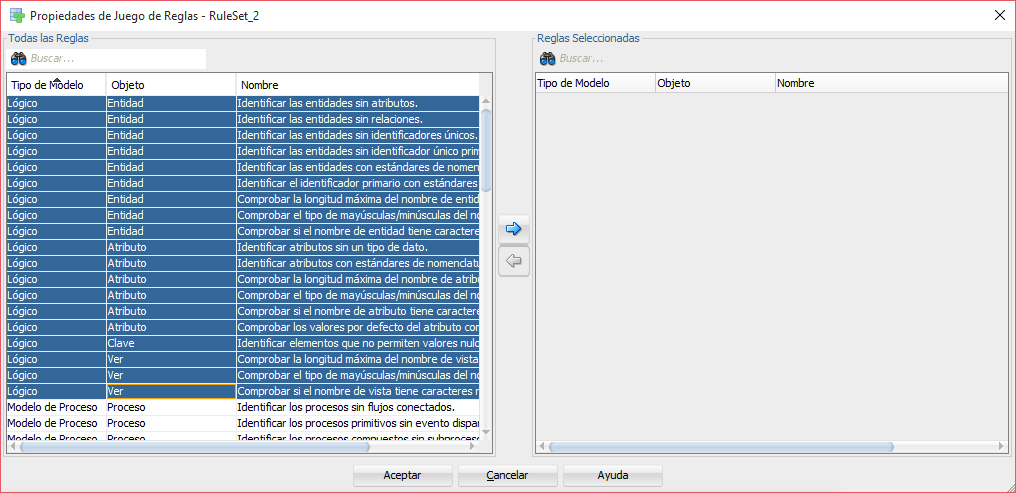
\includegraphics[width=11cm]{./images/5-1 Ejercicio 3/6.png}\\
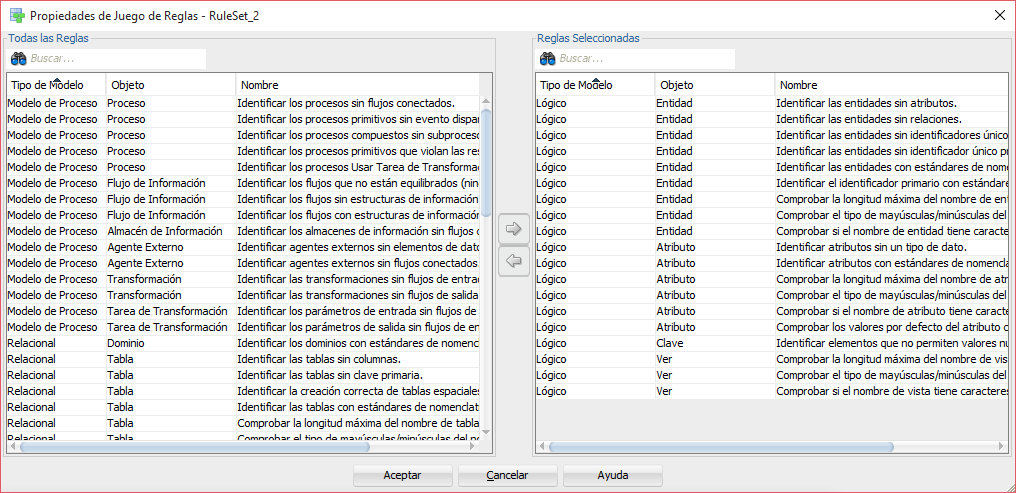
\includegraphics[width=11cm]{./images/5-1 Ejercicio 3/7.png}\\
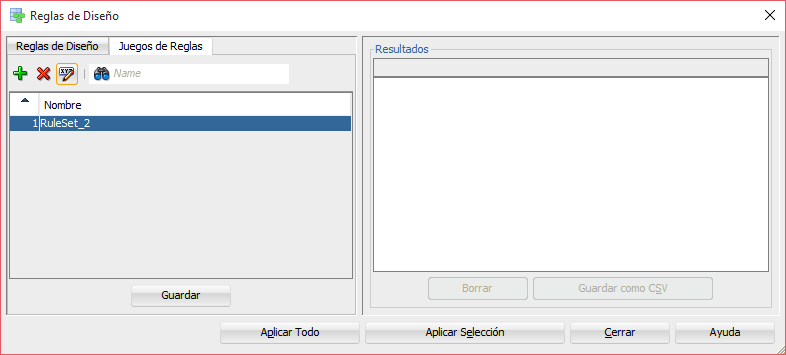
\includegraphics[width=11cm]{./images/5-1 Ejercicio 3/8.png}\\
\end{center}


\section{5-1 Ejercicio 4: Realización de Ingeniería Directa del Diseño para Aplicar el Glosario y el Estándar de Nomenclatura}\label{se:nudo}
\lhead[\thepage/\pageref{LastPage}]{\thesection. Nudo}
\rhead[\thesection. Nudo]{\thepage/\pageref{LastPage}}
Descripción general\\
En esta práctica, realizará ingeniería directa del diseño para aplicar el glosario y el estándar de nomenclatura.\\
Tareas\\
1. Para que el glosario se aplique durante la ingeniería, debe agregarlo en el cuadro de diálogo Preferences
de la página Naming Standard. Para asegurarse de que se aplica el glosario al realizar la ingeniería
directa del modelo, realice los siguientes pasos:\\
\begin{enumerate}
\item Haga clic con el botón derecho en el modelo Design en el explorador y seleccione Properties.
\item Amplíe Settings y haga clic en el nodo Naming Standard.
\item Haga clic en el icono “+” en la región Glossary y navegue hasta la ubicación del glosario.
\end{enumerate}
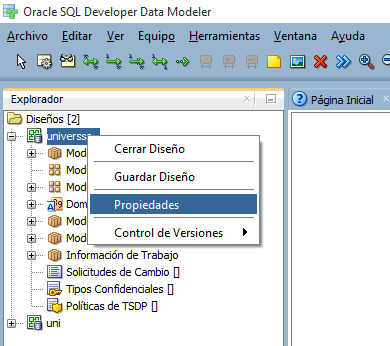
\includegraphics[width=11cm]{./images/5-1 Ejercicio 4/1.png}\\
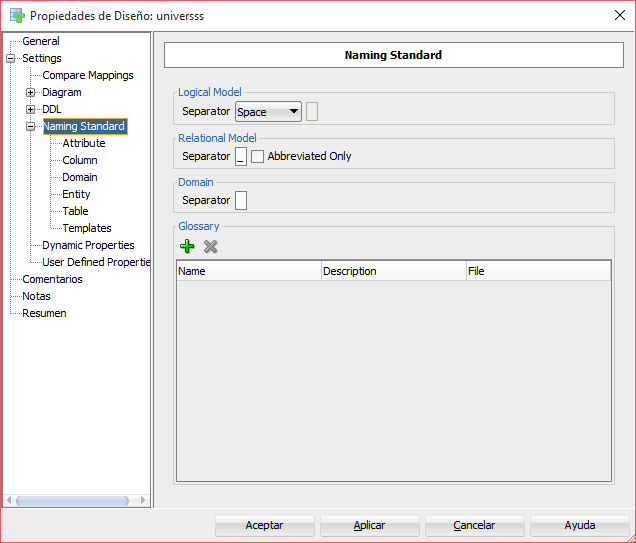
\includegraphics[width=11cm]{./images/5-1 Ejercicio 4/2.png}\\


\section{5-2 Ejercicio 1: Observación de la Asignación de Identificadores Únicos y su Relación en el Modelo Relacional}\label{se:nudo}
\lhead[\thepage/\pageref{LastPage}]{\thesection. Nudo}
\rhead[\thesection. Nudo]{\thepage/\pageref{LastPage}}
Descripción general\\
En esta práctica observará la asignación de los identificadores únicos y su relación en el modelo relacional de la base de datos académica.\\
\begin{center}
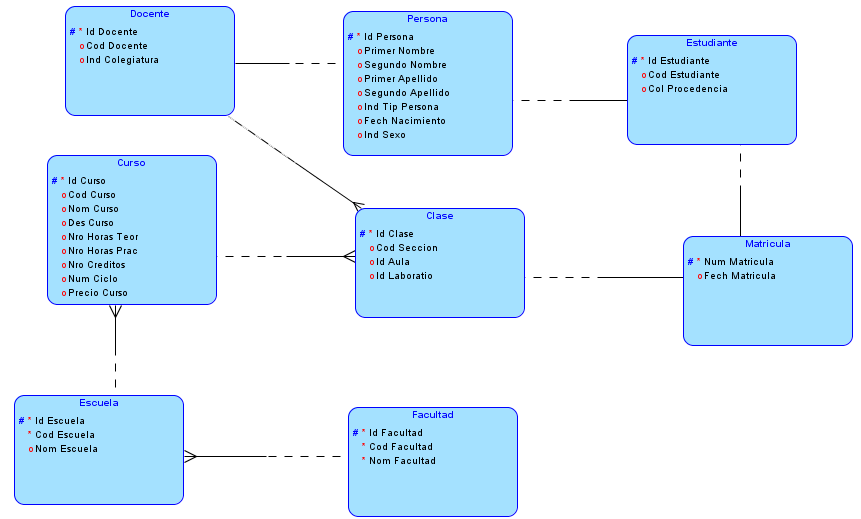
\includegraphics[width=16cm]{./images/5-2 Ejercicio 1/1.png}\\
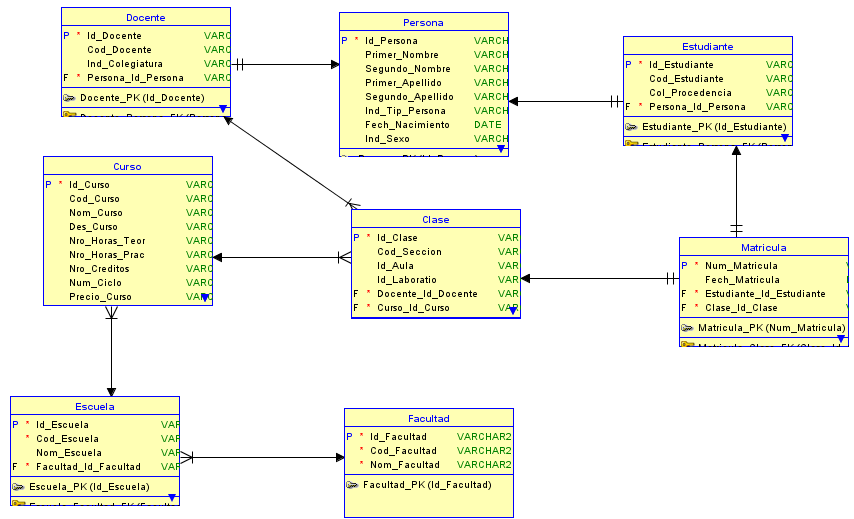
\includegraphics[width=16cm]{./images/5-2 Ejercicio 1/2.png}\\
\end{center}



\section{5-2 Ejercicio 2: Definición de la Plantilla de Nombre}\label{se:nudo}
\lhead[\thepage/\pageref{LastPage}]{\thesection. Nudo}
\rhead[\thesection. Nudo]{\thepage/\pageref{LastPage}}
Descripción general\\
En esta práctica, definirá plantillas (patrones de nombre) para claves, índices y restricciones mediante el uso de combinaciones de variables predefinidas.\\
\begin{center}
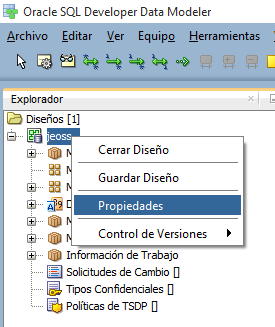
\includegraphics[width=11cm]{./images/5-2 Ejercicio 2/1.png}\\
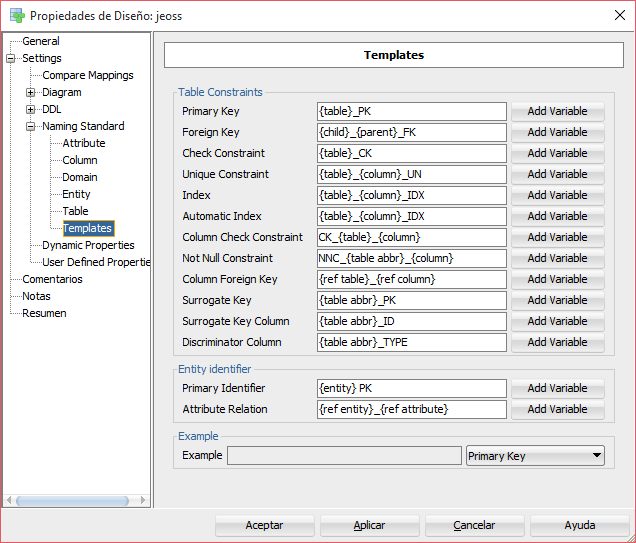
\includegraphics[width=11cm]{./images/5-2 Ejercicio 2/2.png}\\
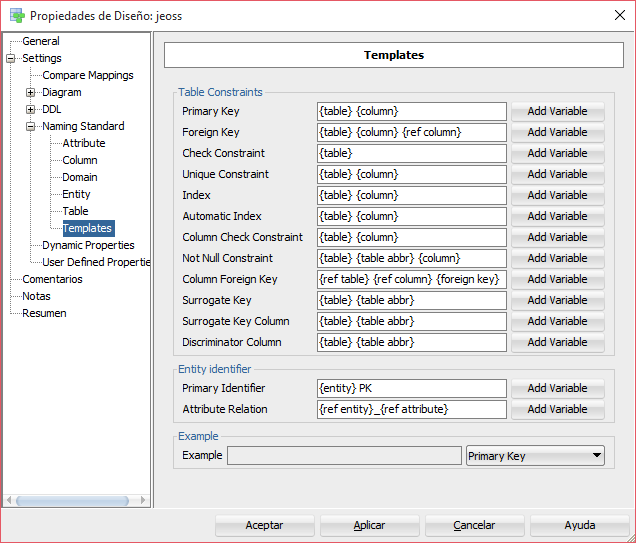
\includegraphics[width=11cm]{./images/5-2 Ejercicio 2/3.png}\\
\end{center}


\section{5-2 Ejercicio 3: Aplicación de Plantilla de Nombre al Modelo Relacional}\label{se:nudo}
\lhead[\thepage/\pageref{LastPage}]{\thesection. Nudo}
\rhead[\thesection. Nudo]{\thepage/\pageref{LastPage}}
Descripción general\\
Después de definir la plantilla de nomenclatura puede aplicarlo a una entidad/tabla o a todo el modelo\\
lógico/relacional. En esta práctica, aplicará la plantilla de nomenclatura a todo el modelo relacional.\\
\begin{center}
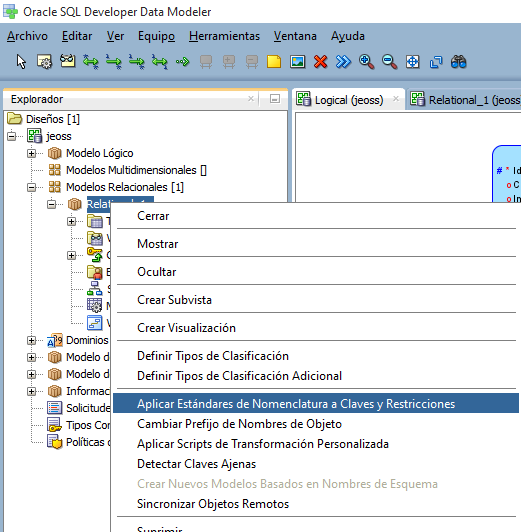
\includegraphics[width=11cm]{./images/5-2 Ejercicio 3/1.png}\\
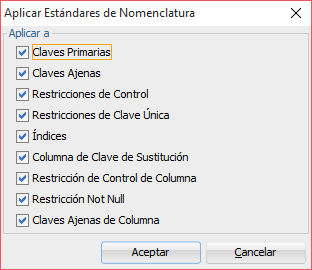
\includegraphics[width=11cm]{./images/5-2 Ejercicio 3/2.png}\\
\end{center}



\section{5-2 Ejercicio 4: Aplicación de un Prefijo de Nombre de Objeto a los Objetos del Modelo Relacional}\label{se:nudo}
\lhead[\thepage/\pageref{LastPage}]{\thesection. Nudo}
\rhead[\thesection. Nudo]{\thepage/\pageref{LastPage}}
Descripción general\\
En esta práctica, aplicará un prefijo de nombre de objeto al modelo relacional de la base de datos académica.\\
\begin{center}
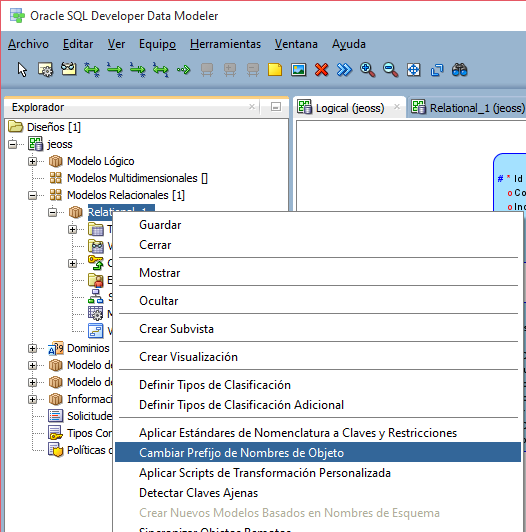
\includegraphics[width=11cm]{./images/5-2 Ejercicio 4/1.png}\\
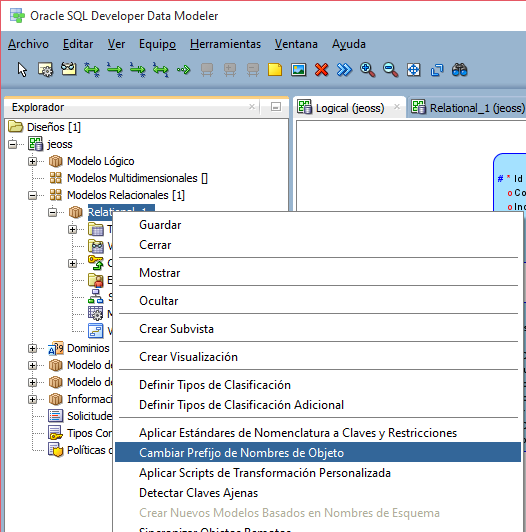
\includegraphics[width=11cm]{./images/5-2 Ejercicio 4/1.png}\\
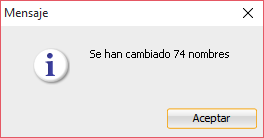
\includegraphics[width=8cm]{./images/5-2 Ejercicio 4/3.png}\\
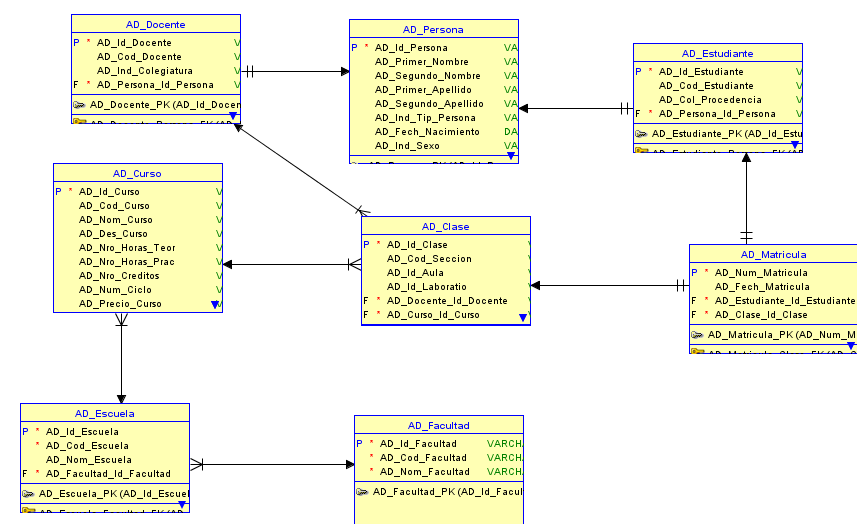
\includegraphics[width=16cm]{./images/5-2 Ejercicio 4/4.png}\\
\end{center}


\section{6-1 Ejercicio 1}\label{se:nudo}
\lhead[\thepage/\pageref{LastPage}]{\thesection. Nudo}
\rhead[\thesection. Nudo]{\thepage/\pageref{LastPage}}
Descripción general\\
En esta práctica, vera un documento que le guiara por las distintas funciones de Oracle Application Express.\\
Tareas:\\
1. Navegue a la Sección 0 de este curso y haga clic para acceder a la Guía del Usuario de APEX.
2. Siga la Guía del Usuario para acceder a Oracle Application Express y conocer las funciones de Oracle Application Express.\\

Ingresamos a traves de la siguiente URL\\
htts://iacademy3.oracle.com\\

Posteriormente nos logeamos\\
\begin{center}
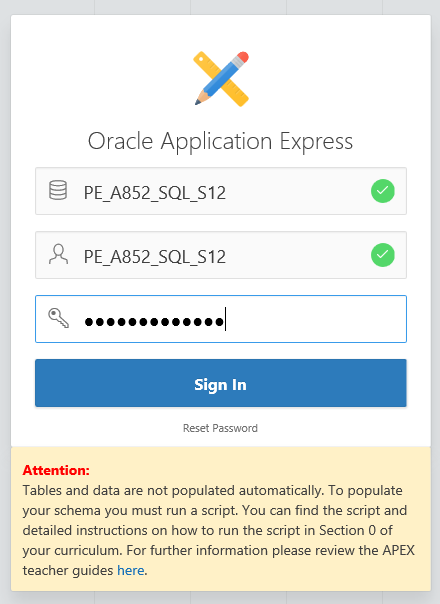
\includegraphics[width=11cm]{./images/6-1 Ejercicio/1.png}\\
\end{center}

Ahora elegimos la siguiente opcion para acceder a las opciones de SQL\\
\begin{center}
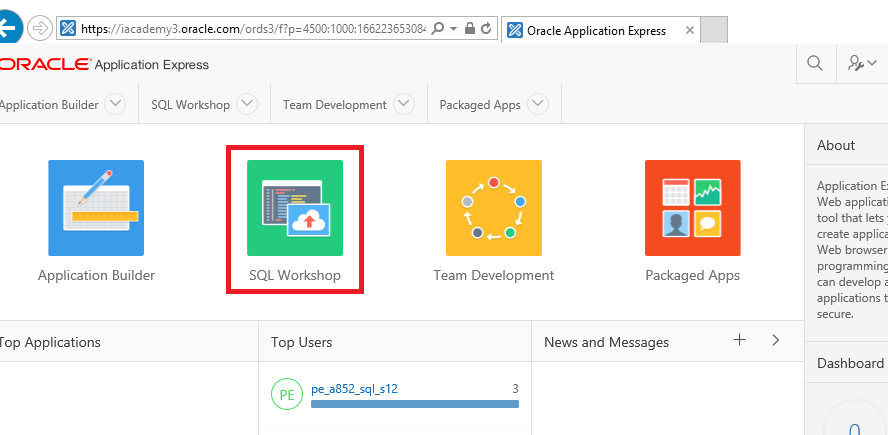
\includegraphics[width=11cm]{./images/6-1 Ejercicio/2.png}\\
\end{center}

Una vez dentro seleccionamos la siguiente opcion para acceder a los comandos SQL\\
\begin{center}
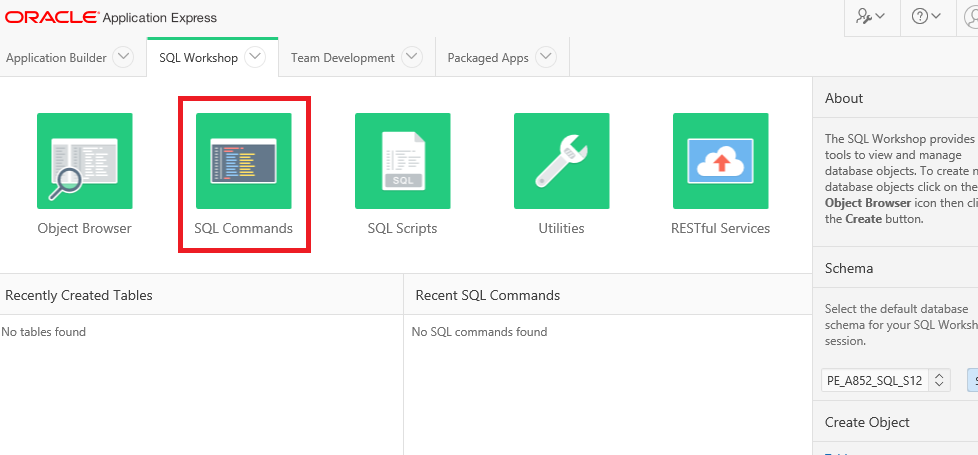
\includegraphics[width=11cm]{./images/6-1 Ejercicio/3.png}\\
\end{center}

Ahi podemos ingresar todas las sentencias SQL para la creacion y modificacion de\\
\begin{center}
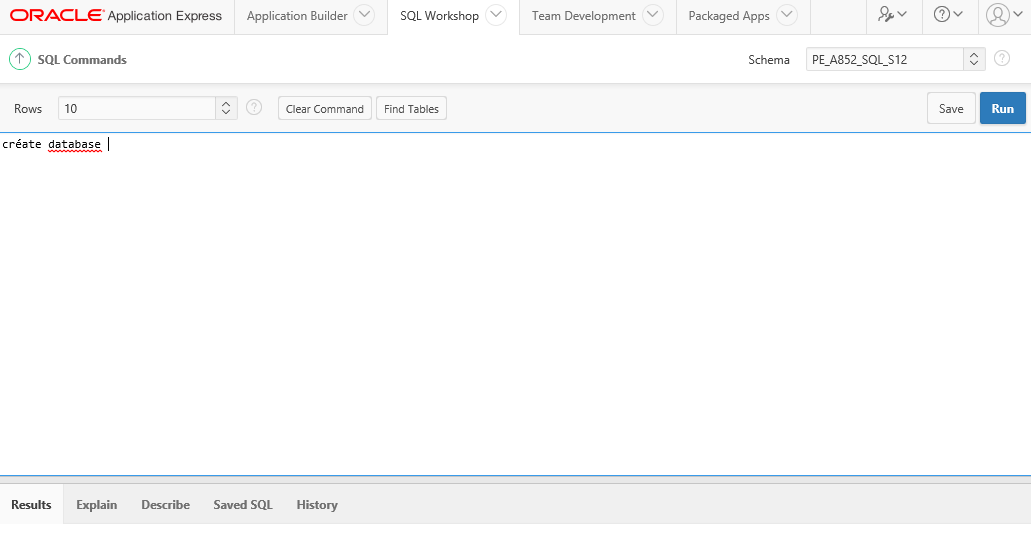
\includegraphics[width=11cm]{./images/6-1 Ejercicio/4.png}\\
\end{center}

En esta parte podremos crear e importar diferentes tipos de aplicaciones\\
\begin{center}
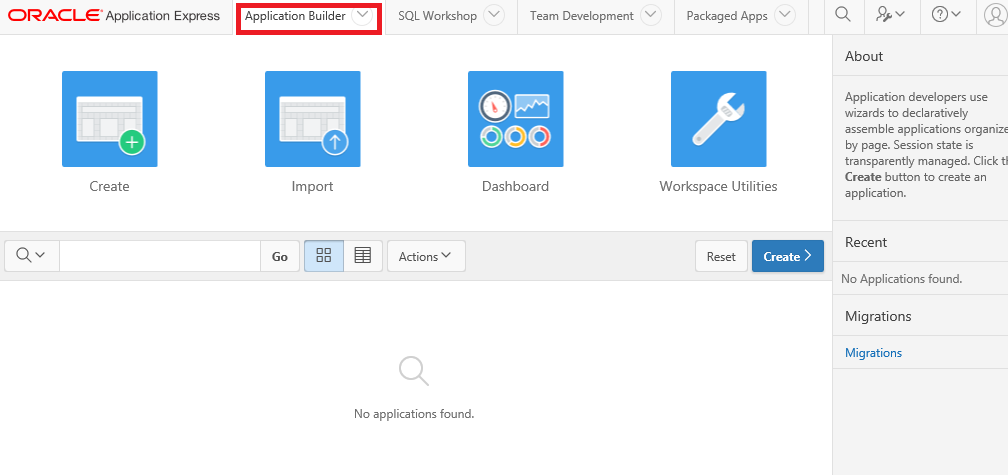
\includegraphics[width=11cm]{./images/6-1 Ejercicio/5.png}\\
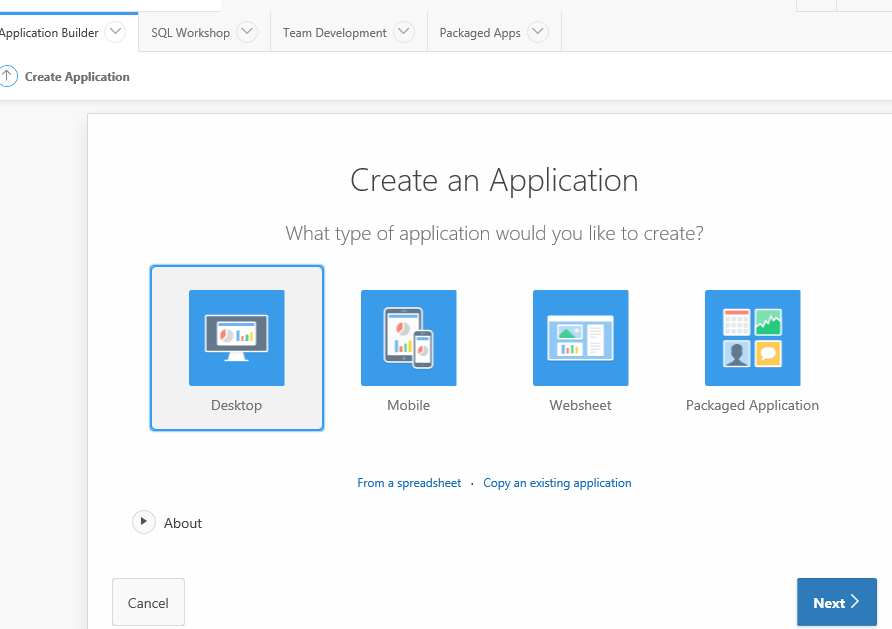
\includegraphics[width=11cm]{./images/6-1 Ejercicio/6.png}\\
\end{center}

\section{6-2 Ejercicio 1}\label{se:nudo}
\lhead[\thepage/\pageref{LastPage}]{\thesection. Nudo}
\rhead[\thesection. Nudo]{\thepage/\pageref{LastPage}}
Descripción general\\
En esta práctica:
• Se conectará a Oracle Application Express
• Se familiarizará con las secciones Help de Oracle Application Express

Supuestos\\
Se le ha asignado un espacio de trabajo de Oracle Application Express y las credenciales para conectarse.\\

Tareas:\\
1. Acceda y conéctese a Oracle Application Express
\begin{enumerate}
\item a. Haga clic en el icono Help y familiarícese con la siguiente sección y temas:
\end{enumerate}
1) Guía del Taller de SQL de Oracle Application Express
\begin{enumerate}
\item Gestión de Objetos de Base de Datos con el Explorador de Objetos
\item Uso de Comandos SQL
\item Uso de Scripts SQL
\end{enumerate}

\begin{enumerate}
\item Haga clic con el botón derecho en el modelo Design en el explorador y seleccione Properties.
\item Amplíe Settings y haga clic en el nodo Naming Standard.
\item Haga clic en el icono “+” en la región Glossary y navegue hasta la ubicación del glosario.
\end{enumerate}

Si ingresamos a la Ayuda de Oracle podremos ver la documentacion respectiva\\
\begin{center}
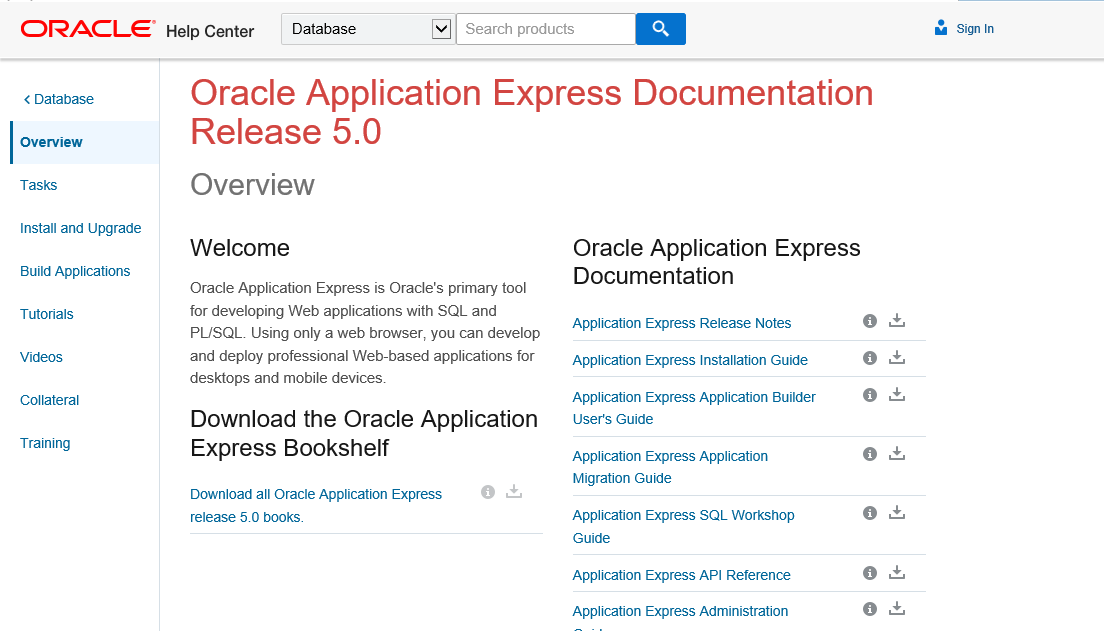
\includegraphics[width=11cm]{./images/6-2 Ejercicio/1.png}\\
\end{center}

Primero ingresamos a las opciones SQL\\
\begin{center}
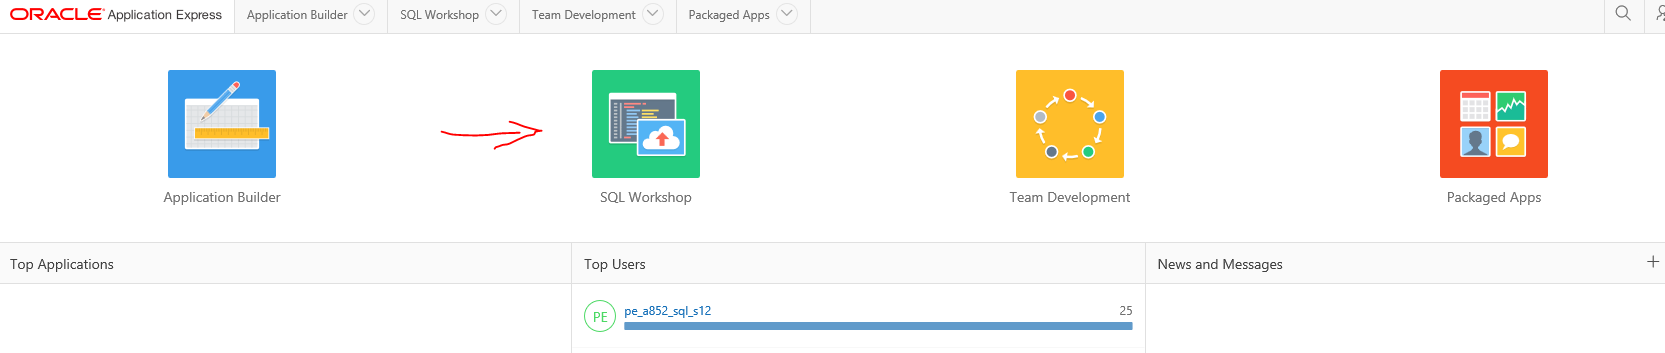
\includegraphics[width=11cm]{./images/6-2 Ejercicio/2.png}\\
\end{center}

Ahora simplemente entramos a las opciones de SQL comandos para poder agregar cualquier tipo de comando SQL\\
\begin{center}
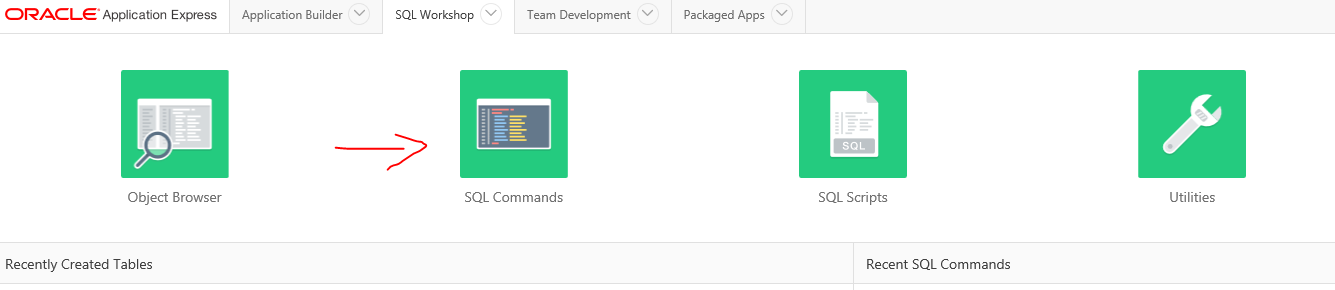
\includegraphics[width=11cm]{./images/6-2 Ejercicio/3.png}\\
\end{center}

Aqui podremos agregar comandos y crea tablas y bases de datose\\
\begin{center}
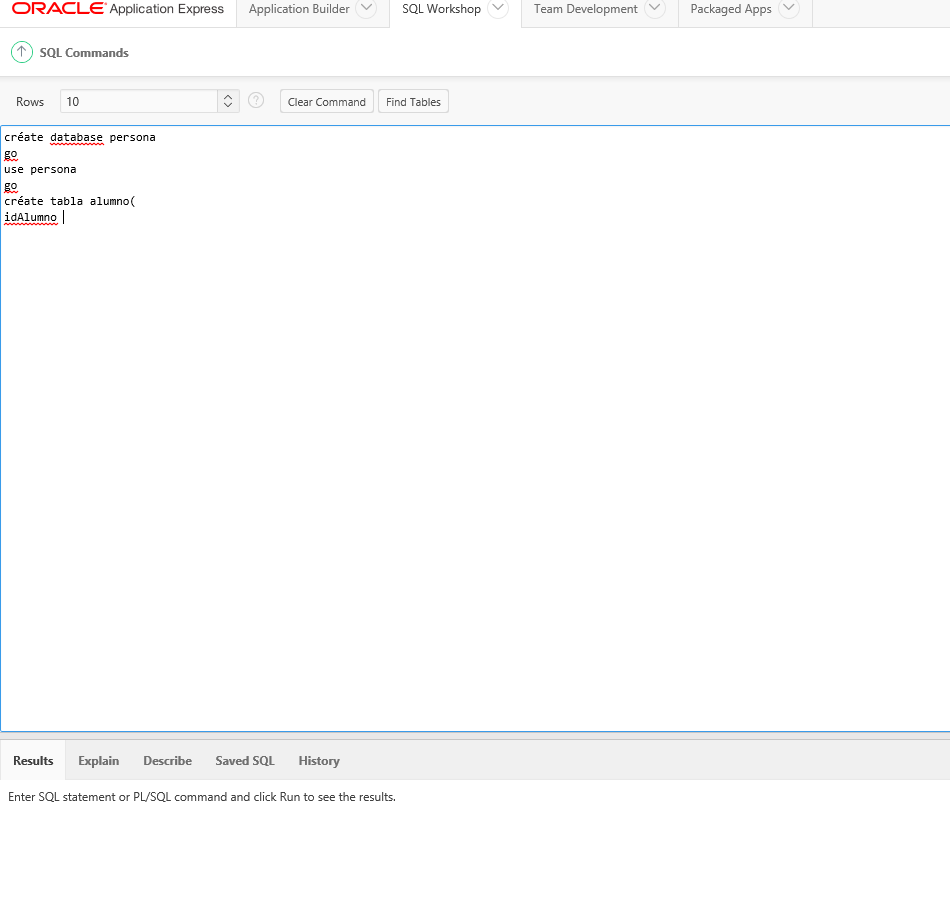
\includegraphics[width=11cm]{./images/6-2 Ejercicio/4.png}\\
\end{center}

Para que podamos usar de Scripts seleccionamos esta opcion y podremos VER los scripts disponibles asi como crear y subir mas scripts\\
\begin{center}
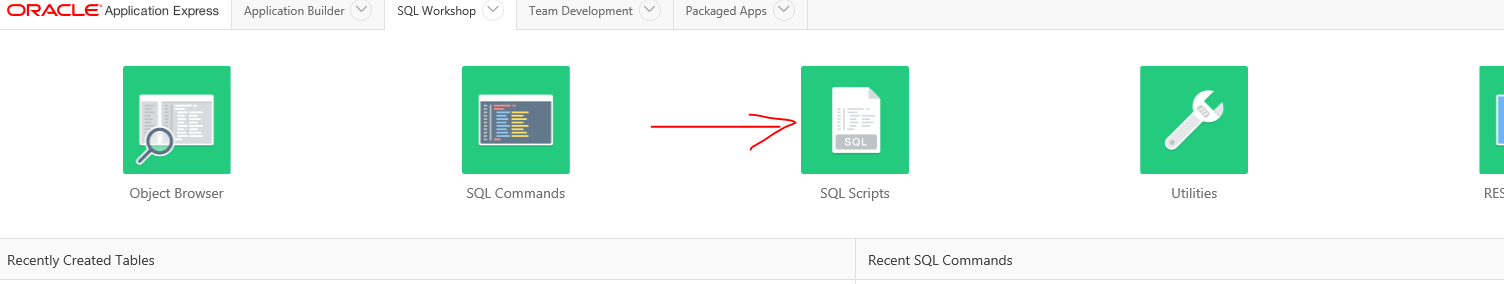
\includegraphics[width=11cm]{./images/6-2 Ejercicio/5.png}\\
\includegraphics[width=11cm]{./images/6-2 Ejercicio/6.png}\\
\end{center}

\section{6-3 Ejercicio 1}\label{se:nudo}
\lhead[\thepage/\pageref{LastPage}]{\thesection. Nudo}
\rhead[\thesection. Nudo]{\thepage/\pageref{LastPage}}

\section{6-4 Ejercicio 1}\label{se:nudo}
\lhead[\thepage/\pageref{LastPage}]{\thesection. Nudo}
\rhead[\thesection. Nudo]{\thepage/\pageref{LastPage}}

\section{6-5 Ejercicio 1}\label{se:nudo}
\lhead[\thepage/\pageref{LastPage}]{\thesection. Nudo}
\rhead[\thesection. Nudo]{\thepage/\pageref{LastPage}}

\section{6-6 Ejercicio 1}\label{se:nudo}
\lhead[\thepage/\pageref{LastPage}]{\thesection. Nudo}
\rhead[\thesection. Nudo]{\thepage/\pageref{LastPage}}

\section{6-7 Ejercicio 1}\label{se:nudo}
\lhead[\thepage/\pageref{LastPage}]{\thesection. Nudo}
\rhead[\thesection. Nudo]{\thepage/\pageref{LastPage}}

\section{6-8 Ejercicio 1}\label{se:nudo}
\lhead[\thepage/\pageref{LastPage}]{\thesection. Nudo}
\rhead[\thesection. Nudo]{\thepage/\pageref{LastPage}}

\section{6-9 Ejercicio 1}\label{se:nudo}
\lhead[\thepage/\pageref{LastPage}]{\thesection. Nudo}
\rhead[\thesection. Nudo]{\thepage/\pageref{LastPage}}



\bibliographystyle{acm} 
\bibliography{biblio}
\addcontentsline{toc}{section}{Bibliografía}
\lhead[\thepage/\pageref{LastPage}]{\thesection. Bibliografía}
\rhead[\thesection. Bibliografía]{\thepage/\pageref{LastPage}}

\end{document}
